\section{Online survey}
\label{sec:online-survey}

Approximately one month after we conducted our first batch of interviews, we
launched an online survey.  After having begun to explore the topic in our
interviews, the purpose of this survey was to obtain a large and diverse number
of responses for a number of specific questions.  We incorporated some of the
preliminary interview data in our survey questions.

\subsection{Method}
\label{sec:survey-design}

We created our survey in Qualtrics because our institution had a subscription,
and it came with all the features that we deemed necessary.  We verified that an
out-of-the-box Tor Browser could correctly take the survey.  However, Qualtrics
requires JavaScript which is deactivated when Tor Browser is set to its highest
security setting.  A number of users complained about the reliance on JavaScript
in the comments of our recruitment blog post~\cite{Winter2017a}.

Our survey was only available in English, but we targeted an international
audience because there are cultural differences in security
behavior~\cite{Sawaya2017a}.  Ignoring these differences would cause us to
optimize Tor Browser's user experience for a predominantly Western audience,
which is problematic.

While we were developing the survey, we used cognitive pretesting (sometimes
also called cognitive interviewing) to improve the wording of our
questions~\cite{Collins2003a}.  Pretesting reveals if respondents \first
understand questions, \second understand questions consistently, and \third
understand questions in the way that we intended.  In our pretests, we administered
our survey and asked the respondents to answer it while verbalizing their thought
process.  We occasionally asked follow-up questions to make sure that our
pretesters understood the questions as intended.  However, not all cognitive
processes can be verbalized, and cognitive pretesting may change the way
respondents answer questions.  We had five pretesters based on whose input we
iteratively improved our survey.  Two pretesters were native English speakers
while the remaining three were fluent but spoke English as a second language.

To weed out low-quality responses we incorporated four attention checks into our
survey~\cite{Berinsky2014a}.  Having four attention checks instead of just one
allows us to measure a respondent's \emph{degree} of attention, meaning that we
only discard responses that failed more than two attention checks.

The majority of our survey focused on onion services, but we also added some
questions about Tor in general.  Table~\ref{tab:survey-structure} shows that our
survey consists of six blocks that are ordered by topic.  It takes about fifteen
minutes to answer all questions.  The full survey is listed in
Appendix~\ref{app:interview-questions}.  Finally, we launched our survey on
August 16, 2017 and ended it on September 11, 2017, so it was active for 27
days.

\begin{table}[t]
	\centering
	\begin{tabular}{l r}
	\toprule
	Topic & \# of questions \\
	\midrule
	Consent and demographic information & 1 \\
	Tor usage & 4 \\
	Onion site usage & 20 \\
	Onion site operation & 5 \\
	Onion site phishing and impersonation & 9 \\
	Expectations of privacy & 9 \\
	End of survey & 1 \\
	\midrule
	Total & 49 \\
	\bottomrule
	\end{tabular}
	\caption{The topical question blocks in our survey and the number of
	questions they contain.}
	\label{tab:survey-structure}
\end{table}

\subsubsection{Recruitment}

Similar to our interviews, we advertised our survey in a blog post on The Tor
Project's blog~\cite{Winter2017a}, on its corresponding Twitter account, and on
three Reddit subforums.\footnote{The forums are \url{https://reddit.com/r/tor/},
\url{https://reddit.com/r/onions/}, and \url{https://reddit.com/r/samplesize/}.}
Again, note that this recruitment strategy is likely to bias our sample towards
more engaged users as casual Tor users are unlikely to follow The Tor Project's
blog or Twitter account.

\subsubsection{Research ethics}
Respondents had to agree to a consent form before starting the survey. The
consent form informed the respondents about the procedure of our experiment and
verified that all respondents were at least eighteen years of age.

To provide additional incentives, we originally planned to give respondents the
option to participate in a gift card lottery.  We abandoned the idea because it
was non-trivial to reconcile a lottery with anonymous participation because we
would have to collect our respondents' email addresses.  Despite the lack of
incentives, we collected a sufficient number of responses.  In fact, we believe
that many of our respondents were primarily motivated by improving Tor---some of
our interview participants turned down the gift cards that we offered.

\subsection{Results}
\label{sec:results}

Throughout all 27 days, our survey was taken 828 times.  However, not all
responses are necessarily of high quality; people may have rushed their answers,
aborted our survey prematurely, or given deliberately wrong answers.  We weed
out such low-quality responses that \first did not finish the survey and that
\second failed more than two out of our four attention checks.  We collected a
total of 828 responses but only 604 (73\%) completed the survey and 527 (64\%)
passed at least two attention checks.  The remainder of this section analyzes
these 527 responses.

Table~\ref{tab:survey-demo} shows the demographics of our survey.  Not
surprisingly, our respondents were \emph{young and educated}: more than sixty
percent are younger than 36, and another sixty percent have at least a graduate
degree.  Finally, another sixty percent consider themselves at least highly
knowledgeable in matters of Internet privacy and security.

\begin{table*}[t]
	\centering
	\begin{tabular}{l r l r l r l r}
	\toprule
	Gender & \% &
	Age & \% &
	Education & \% &
	Domain knowledge & \% \\
	\midrule
	Female & 8.9  & 18--25   & 35.5 & No degree     & 5.5  & No knowledge             & 0.5  \\
	Male   & 86.3 & 26--35   & 34.6 & High school   & 31.9 & Mildly knowledgeable     & 7.6  \\
	Other  & 4.8  & 36--45   & 17.5 & Graduate      & 42.3 & Moderately knowledgeable & 32.4 \\
	       &      & 46--55   & 8.7  & Post graduate & 20.4 & Highly knowledgeable     & 44.9 \\
	       &      & 56--65   & 2.5  &               &      & Expert                   & 14.6 \\
	       &      & $>$ 65   & 1.2  &               &      & & \\
	\bottomrule
	\end{tabular}
	\caption{The distribution over gender, age, education, and domain knowledge 
	for our 621 interview subjects.}
	\label{tab:survey-demo}
\end{table*}


\subsubsection{Biases}

As mentioned earlier, it is very difficult to draw a truly uniform sample of Tor
users.  The only way to reach all Tor users uniformly would be to modify Tor
Browser's landing page that is displayed on start.  Unfortunately, this approach
is very invasive.  We opted for asking The Tor Project to disseminate our survey
on its blog and social media accounts.  We believe that this recruitment
strategy came with the following biases.

\begin{description}
    \item[Survivor bias] We predominantly heard from people who can tolerate
        Tor's usability issues enough to still be around and take a survey on
        the topic.  We likely did not hear from many---if any---people who gave
        up on Tor and are no longer around to tell their tale.  The danger of
        survivor bias lies in optimizing the user experience for the subset of
        people who could tolerate a bad user experience.

    \item[Self-selection bias] Due to the nature of our online survey,
        participants could voluntarily select themselves into the group of
        respondents. \textbf{TODO}
        No paranoid people or people who don't like
        JavaScript.  Not a huge problem as we know how they think.  We also
        mostly reached people who are unusually engaged.
\end{description}

\subsubsection{Tor usage}

Our survey started with two general questions about the use of Tor Browser.
Figure~\ref{fig:tor-usage} illustrates how often our respondents use Tor
Browser.  Almost half of our participants use Tor Browser either daily or even
as their main browser.

Figure~\ref{fig:tor-threats} illustrates what entities our respondents seek to
protect themselves from when using Tor Browser.  The majority considers ad
companies, governments, and---most prominently---their ISP.  More relatable
entities such as family, employer, and school are less prevalent.

\begin{figure}[t]
    \centering
    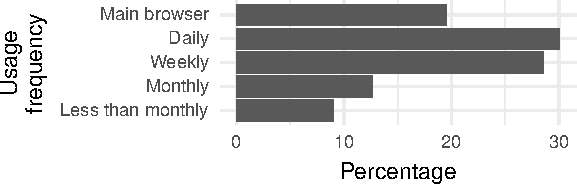
\includegraphics[width=\linewidth]{figures/tor-usage.pdf}
    \caption{The usage frequency of Tor Browser among our respondents.  Almost
    half of our respondents use Tor Browser either daily or as their main
    browser.}
    \label{fig:tor-usage}
\end{figure}

\begin{figure}[t]
    \centering
    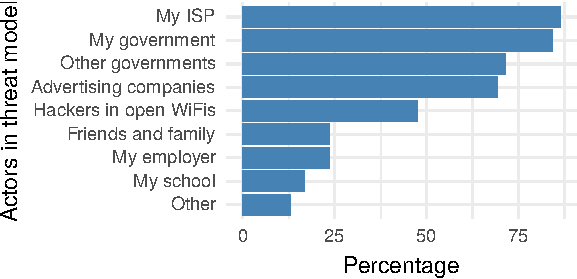
\includegraphics[width=\linewidth]{figures/tor-threats.pdf}
    \caption{The threat actors that our respondents seek to protect themselves
        from by using Tor Browser.}
    \label{fig:tor-threats}
\end{figure}

People who selected ``Other'' gave a variety of responses.  A number of
respondents specifically pointed out Google and Facebook.  ISPs, backbone ISPs,
and websites were another common theme.  A number of respondents are struggling
with personal threats that include identity theft, targeted harassment, and
stalking.  Research is another common theme: Several respondents want to learn
about a topic without revealing their interest in it.  Some respondents use Tor
for search engine optimization, computer security research, and to research
medical conditions.  Finally, Tor provides technical advantages that don't
involve a threat actor.  Some respondents want IPv6 connectivity, evasion of
geographical content restrictions, and access to onion services.  A small number
of respondents are only interested in technical aspects other than privacy.  One
respondent stated that they don't need anonymity themselves but instead use Tor
to provide cover traffic for ``people who need protection.''

\subsubsection{Onion service usage}

The usage frequency of onion services is almost uniformly distributed among our
respondents; 24\% use onion sites less than once a month, 22\% use them about
monthly, 25\% weekly, and 23\% daily.  The remaining 6\% has never used an onion
service before.

The majority of our respondents (61.8\%) has used onion services for purposes
other than web browsing before.  Several protocols such as the chat application
Ricochet~\cite{ricochet} and the file sharing application
OnionShare~\cite{onionshare} were purpose-built on top of onion services while
existing TCP-based tools such as SSH can also be used with onion addresses
instead of traditional IP addresses.  Almost one third (29.7\%) of our
participants use onion service for non-browsing activities at least once a week.

But why do Tor users browse onion services in the first place?
Figure~\ref{fig:onion-usage} provides an answer.  The majority uses onion
services because of the additional anonymity (70\%) and the additional security
(61\%).  For 46\% it is the only way to access some content they enjoy, so using
onion services is a necessity.  27\% of our respondents found themselves curious
about the ``Dark Web'' and set out to find their own answer and 19\%
occasionally stumble upon links to onion services in their day-to-day browsing
activity.  Respondents who selected ``Other'' gave a variety of reasons, the
most predominant of which was the ability to set up a TCP service behind a NAT
device.  That way, it is possible to run an SSH server in a home network that
has neither a permanent IP address, nor port forwarding.  Other noteworthy
respondents use onion services to reduce the load on exit relays, to do
technical research, and to access sites that are otherwise unavailable.

\begin{figure}[t]
    \centering
    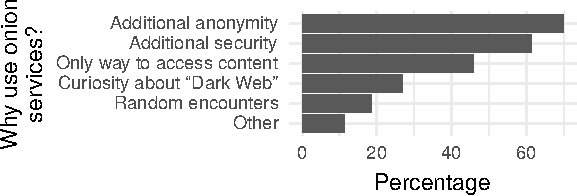
\includegraphics[width=\linewidth]{figures/onion-usage.pdf}
    \caption{Our respondents' (multiple choice) reasons for using onion
    services.}
    \label{fig:onion-usage}
\end{figure}

\subsubsection{Onion service discovery}

Recall that onion services are private by default, leaving it up to their
operator to disseminate the domain.  Established search engines such as Google
are therefore inadequate to find content on onion services.  We wanted to find
out how our respondents discover onion services.
Figure~\ref{fig:onion-discovery} illustrates the results.  The three most
popular ways of discovering new onion sites, all approximating 50\%, are social
networking sites such as Twitter and Reddit, the list of search engines such as
Ahmia\footnote{Ahmia.fi is an onion site search engine that crawls
user-submitted onion domains.  It publishes the list of all indexed onion
services at \url{https://ahmia.fi/onions/}.}, and randomly encountering links
when browsing the web.

While significantly less popular, discovering onion domains through friends and
family has the advantage of trust.  Some of our interview participant indicated
that they heavily rely on this distribution method simply because they can trust
the origin.  Finally, a mere 4\% indicated that they are not interested in
learning about new onion services.

Respondents who selected ``Other'' predominantly brought up
independently-maintained lists of onion services and aggregators.  A noteworthy
example is the Hidden Wiki.

\begin{figure}[t]
    \centering
    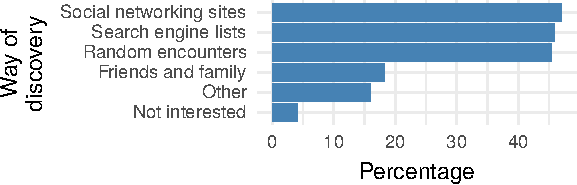
\includegraphics[width=\linewidth]{figures/onion-discovery.pdf}
    \caption{Our respondents' (multiple choice) methods of discovering onion
    services.}
    \label{fig:onion-discovery}
\end{figure}

The next question in our survey then asked if our respondents are satisfied with
the way they discover onion services.  60\% selected ``Yes'' while 40\% selected
``No.'' Some respondents who selected ``Yes'' brought up that they have no
interest in learning about new onion services, in part because they only use a
small set of onion services.  Among the people who are not satisfied, the most
prominent complaint was about broken links on onion site lists.  There is
non-trivial churn among onion sites and our respondents were frustrated that
existing lists are typically not curated and contain many dead links.

Many respondents were not aware of search engines such as ahmia.fi.  Among those
that were, many were not satisfied with both the search results and the number
of indexed onion sites.  Unsurprisingly, a ``Google for onion sites'' was a
frequent wish.

Several respondents were unhappy with existing aggregators.  In addition to
broken links, some distrust lists because they occasionally contain scam and
phishing sites.  The difficulty of telling apart two given onion domain names
exacerbates this issue.  Another common wish for aggregators was for them to be
more verbose in their description of onion sites.  In particular, some
respondents want to avoid illegal and pornographic content, which is often
difficult if the description is vague and the onion domain reveals nothing about
its content.

Many respondents expressed frustration about the difficulty of finding out if
site X also provides a corresponding onion service.  A common wish was to have
site X list its onion service prominently in a footer.  Ironically, some
respondents were surprised that torproject.org has a corresponding onion site --
they couldn't find it on the web site.

Interestingly, some respondents voiced frustration about various usability
issues, but mentioned in the same sentence that this is an inherent trade-off of
privacy technology, suggesting that there is nothing that can be done about it.

\subsubsection{Onion service domain format}

Conventional domains are designed to be easy to remember and recognize.  But how do users
handle the randomly-generated onion domains?  Question 3.8 in our survey asked
exactly that, with the responses being illustrated in
Figure~\ref{fig:onion-domain-mgmt}.

\begin{figure}[t]
    \centering
    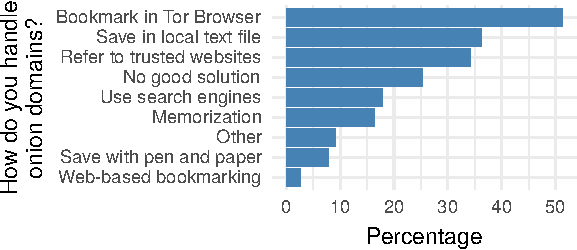
\includegraphics[width=\linewidth]{figures/onion-domain-mgmt.pdf}
    \caption{The strategies that our respondents use to handle onion domains.
    More than half use bookmarks inside of Tor Browser and a quarter thinks that
    there's no good solution.}
    \label{fig:onion-domain-mgmt}
\end{figure}

Most respondents use bookmarks inside Tor Browser for onion domains.  While
convenient, it leaves a trace of (presumably) visited sites on one's computer.
One of Tor Browser's security requirements is ``disk avoidance,'' \ie, the
browser must not write anything to disk that would reveal the user's browsing
history~\cite[\S~2.1]{Perry2017a}.  Bookmarking links is a violation of this
security requirement.  Many of our respondents were aware of this issue.  About
a dozen respondents who selected ``Other'' stated that they store onion domains
encryptedly---either in a text file or in their password manager.

Somewhat less popular is saving onion domains in local text files (36\%),
getting them from trusted websites (34\%), use search engines (18\%), memorize
domains (16\%), use some other techniques (9\%) or employ pen and paper (8\%).
Notably, one quarter of our respondents does not have a good solution to the
problem.  Given the alarming number of (possibly insecure) home-baked solutions,
a Tor Browser extension may be warranted to approach the problem.

The next question in our survey asked if our respondents expect the
next-generation domain format to change their browsing habits.  Interestingly,
only 17\% expect to have their browsing habits changed while 83\% don't.  Among
the respondents who selected ``Yes,'' many expressed that they memorize a small
number of onion domains (such as Facebook's), which will no longer be possible.
People who selected ``No'' mostly bring up that they treat onion domains as
opaque identifiers that they handle via tools such as bookmarks.  These results
suggest that the current state is dire, yet not expected to get much worse with
the new domain format.

Problematic:
``I only memorize the first part of the domain''

``If there isn't some cognizable word at the start, it'll be more difficult for
me to determine if I'm going to the correct domain or a scam. I may end up going
to less .onion sites as a result.''

\subsubsection{Onion service operation}

A survey question block on onion service operation shed light on the reasons for
running onion services and what sort of issues users face when doing so.  40\%
of our respondents once set up an onion service.  Among the respondents who
never have, 31\% have considered doing so while 30\% have never even considered
it.  Interestingly, 79\% of operators have run an onion service for private use
while 53\% have run them for the public.

Figure~\ref{fig:onion-operation-reasons} gives an overview of the reasons for
running onion services.  Interestingly, the extra security properties overshadow
the anonymity properties of onion services.  Another particularly popular reason
is NAT traversal---many respondents noted that onion services allow them to
expose a TCP service in their home network despite being behind a NAT device.
Finally, some people run onion service indirectly because third-party tools such
as OnionShare~\cite{onionshare} or Ricochet~\cite{ricochet} are built on top of
them.  Onion services can have clear benefits for businesses as well as
evidenced by one respondent who wrote on onion services: ``We use it for
delivering updates to our router to customers securely and without leaking
metadata.''

\begin{figure}[t]
    \centering
    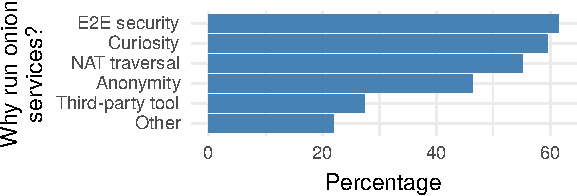
\includegraphics[width=\linewidth]{figures/onion-operation-reasons.pdf}
    \caption{The reasons people have for running onion services.}
    \label{fig:onion-operation-reasons}
\end{figure}

Figure~\ref{fig:onion-operation-concerns} illustrates the concerns that onion
service operators face.  We consider three attacks; \first somebody setting up a
phishing site for the operator's site, \second a denial-of-service attack, and
\third a deanonymization attack.  More than half of our respondents are at least
somewhat concerned about all of these attacks.  Almost 40\% claim to be
extremely concerned about somebody deanonymizing their onion service.  Indeed,
many respondents lamented the difficulty of knowing that an onion service setup
is robust against application-layer deanonymization attacks.

\begin{figure}[t]
    \centering
    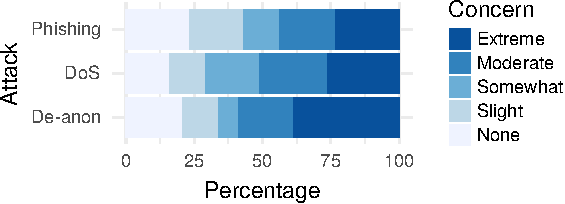
\includegraphics[width=\linewidth]{figures/onion-operation-concerns.pdf}
    \caption{The level of concern onion service operators have with respect to a
    phishing clone of their service, denial-of-service attacks, and
    deanonymization.}
    \label{fig:onion-operation-concerns}
\end{figure}

\subsubsection{Susceptibility to phishing attacks}

Phishing remains an issue despite onion services' extra anonymity and security
properties.  Past work has uncovered an attack that transparently rewrote
Bitcoin addresses to hijack Bitcoin
transactions~\cite{Winter2016a,Nurmi2015a,Monteiro2016a}.  Key to this attack is
the difficulty of telling apart an authentic from an impersonation domain.  For
conventional domains we rely on (EV) certificates, browser protections, search
results, and long-lived reputation, but none of these methods work well for
onion services.  Does the nature of onion services facilitate phishing attacks?
If so, what can we do to mitigate the issue?

We asked our respondents if they ever thought about the authenticity of an onion
site.  With 80\%, the majority of our respondents did while 20\% didn't.
Clearly, there is a need for verification but how does one verify that an onion
service is authentic?  Figure~\ref{fig:determining-legitimacy} gives an overview
of the strategies that our respondents employ.

\begin{figure}[t]
    \centering
    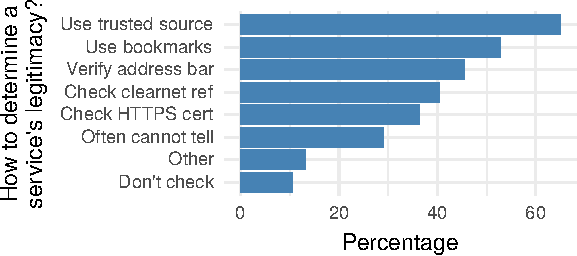
\includegraphics[width=\linewidth]{figures/determining-legitimacy.pdf}
    \caption{How our respondents determine an onion service's legitimacy.}
    \label{fig:determining-legitimacy}
\end{figure}

More than half either consult trusted sources (\eg friends or another web site)
or use bookmarks when revisiting onion services.  Many respondents also verify
the domain in the browser's address bar (46\%), check if the corresponding web
site has a link to its onion site (41\%), or hope that the onion service has an
HTTPS certificate (36\%).\footnote{DigiCert is issuing EV-certificates for onion
sites~\cite{DigiCert2015a} but adoption has been slow---presumably in part
because EV certificates require the CA to verify the applicant's identity
and they are not for free.}  Alarmingly, almost 30\% of respondents stated that
they sometimes cannot tell the difference between an authentic service and an
impersonation, and 11\% never check a service's legitimacy in the first place.
People who selected ``Other'' provided a wide variety of ad-hoc phishing
protections---some clearly misguided, which reinforces the scope of the problem.

Originally meant to improve usability, vanity onion domains also play a role in
the context of phishing.  There is concern that the short and recognizable
prefixes tempt users to only verify the prefix and ignore subsequent
characters~\cite{Winter2015a}.  This oversight may allow attackers to create
impersonation domains that feature the prefix but differ in subsequent
characters.  Nurmi~\cite{Nurmi2015a} and Monteiro~\cite{Monteiro2016a} have both
documented such an attack but its effectiveness is not known.

The majority of our respondents appreciates vanity domains because they are easy
to remember (64\%), easy to recognize (64\%), and they provide a unique
``branding'' (34\%).  Some responses indicate that a vanity prefix conveniently
informs about an onion service's topic, letting visitors know what to expect.
Only 8\% dislike vanity onion domains and 15\% don't have an opinion.
Interestingly, some respondents consider vanity domains unfair because wealthy
entities can afford to generate longer prefixes.  Several respondents voiced
their concern that vanity domains create a false sense of security and
facilitate phishing attacks.  In a separate question we inquired how many
characters our respondents verify in onion domains.  43\% verify 13--16 digits,
\ie (almost) the full domain, while 46\% verify up to nine digits, which is
within the realm of brute force attacks.  Finally, a handful number of
respondents cited misguided reasons why they dislike vanity domains, \eg some
believe that vanity domains are a sign of weak hash functions while others
believe that vanity domains make the onion service ``less hidden'' or allow
somebody to create ``the same private key.''
